\problemname{Snow Wall}
After the humiliation in the snowball fight, Sweden plans to build a snow wall, and force Finland to pay for it.
The wall shall have a certain width $W$, and be as tall as possible (it's going to be \emph{yuuuge}!).

As building material, there are a number of snow blocks that all have height 1, but can have different widths.
When the wall is constructed, each block must satisfy the following rule: on the row below the block,
at the two positions where the block has its endpoints, there must be a block immediately to the right and left of the point,
except at the beginning and end of a row, where there must instead be an endpoint \emph{on every row}.

Furthermore, there must not be a gap at the same position on two directly consecutive rows \emph{in the wall} (the empty row
just above the wall does not count).

The following image illustrates some invalid (left) and valid (right) walls:

\begin{figure}[h]
	\centering
	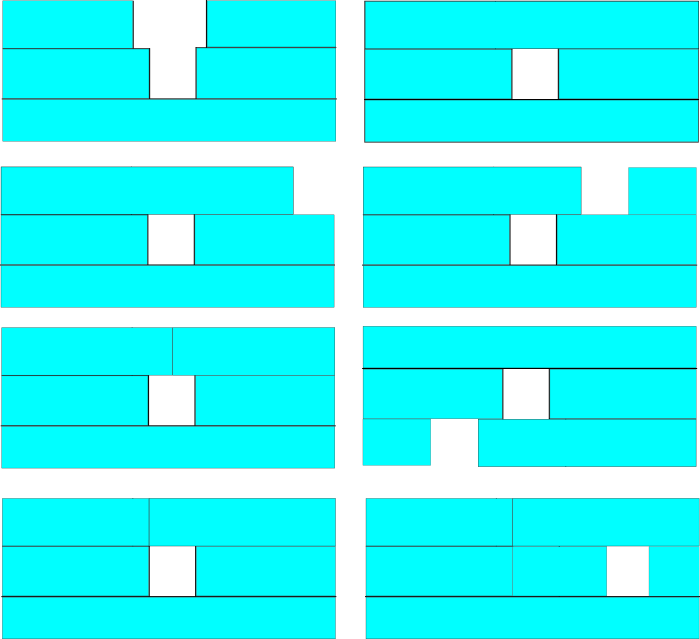
\includegraphics[width=0.7\textwidth]{mur.png}
	\caption{A number of invalid (left) and valid (right) walls.}
\end{figure}

Given the width $W$ and the available blocks, construct as tall a wall as possible.

\section*{Input}
\textbf{Note:} the test data for this problem is open. You can download it in the attachments or \href{https://progolymp.se/uploads/snomur.zip}{here}.

\noindent
The first line contains three integers $T$, $N$, and $W$ --- the test case number, the number of blocks, and the width of the wall.
The next line contains $N$ integers, the width of each block.

\section*{Output}
On the first line, output the height of your wall, $H$.

Then output $H$ lines, one for each row of your wall.
Line $i$ shall first have a number $B$, the number of blocks on that row of your wall.
This shall be followed by $B$ pairs of integers $P_{i,j}, L_{i,j}$, the position and length of the $j$th block on the row.

\section*{Submission}
When submitting your solution, it suffices to have a program that reads the test case number $T$ and outputs the solution for that test case.

If you do not want to write such a program yourself, you can use a page we constructed: \url{http://progolymp.se/uploads/snokaosgen.html} where you can paste
all your solutions and get a Python 3 program that you can submit.

\section*{Scoring}
Your program will be tested on test cases, and scored based on how it compares to the judges' solution.

Assume that on a test case your program achieves height $X$, and the judges' solution achieves height $Y$. Then you get $10 \times \frac{X}{Y}$ points on the test case, rounded to two decimal places.

Your score for a submission is the sum of the scores for the test cases, and your total score is the score of the best submission. It is thus not possible to combine test cases between different submissions; you must submit a single program that maximizes your score on all test cases simultaneously.

Your solution can receive at most $100$ points, even if it is better than the judges' solution.
